% !TEX root =../LibroTipoETSI.tex
\chapter{Denegación de Servicio}\LABCHAP{Denegacion de Servicio}
\pagestyle{esitscCD}
\epigraph{ Denial of Service: ``The prevention of authorized access to resources or the delaying of time critical 
operations''. }{ITU-T recommendation X.800}

%\lettrine[lraise=0.7, lines=1, loversize=-0.25]{E}{l} 
\lettrine[lraise=-0.1, lines=2, loversize=0.25]{E}n este capítulo trataremos de definir qué es un \gls{DoS} 
\index{DoS}, qué significa que un ataque de denegación de servicio sea distribuido \acrshort{DDoS} \index{DDoS}, por 
qué es importante su prevención, por qué es tan difícil su identificación y defensa, esto es, la motivación del 
proyecto.

Las diferentes secciones seguirán la misma clasificación que siguen S.V. Raghavan y E. Dawson en su libro ``An 
Investigation into the Detection and Mitigation of Denial of Service (DoS) Attacks'' \cite{Raghavan}. Trataremos de 
definir qué es un ataque \gls{DoS} en la \SEC{Definicion DoS}, y qué significa que un ataque \gls{DoS} sea 
distribuído en la sección \gls{DDoS}. Tras ello, diseccionaremos los distintos tipos, a fin de obtener una visión 
general pero suficiente de las formas de llevarlo a cabo, en la \SEC{Taxonomia DoS}.

Por último, con toda la información adquirida en los apartados nombrados, seremos capaces de estudiar la detección y 
posible mitigación de los distintos tipos en la sección \SEC{Deteccion y mitigacion DoS}.

%http://en.wikibooks.org/wiki/LaTeX/List_Structures#Customizing_Lists
\section{Definición y consecuencias de un ataque de denegación de servicio} \LABSEC{Definicion DoS}
La seguridad de la información se puede dividir en tres sectores: confidencialidad, esto es, la 
información sólo es vista por los destinatarios; integridad, esto es, la información no ha sido 
alterada desde que se registró y, por último, disponibilidad: El destinatario puede obtener la 
información siempre que la necesite. Un sistema es seguro en la medida que cumple estas tres 
condiciones.

La definición formal que ofrece la \gls{ITU-T} en su recomendación X.800 es la siguiente \cite{ITU-T_DDoS_def}:

\begin{quote}
 The prevention of authorized access to resources or the delaying of time critical operations.
\end{quote}

Por su parte, el \gls{CNSS} ofrece una definición más general \cite{CCNS_DDoS_def}:

\begin{quote}
 Any action or series of actions that prevents any part of an information system from functioning.
\end{quote}

Así pues, los ataques de denegación de servicio atacan directamente a la disponibilidad. Esta falta de disponibilidad 
pueda ser debida a acciones maliciosas o no, originadas de manera local al sistema que se desea proteger o remotamente.

Para impedir el acceso a los recursos, el atacante puede atacar cualquier eslabón de la cadena: Desde el ancho de banda 
de la red que conecta el usuario con el mismo, la memoria o capacidad de procesamiento de la que dispone el sistema, 
alguna debilidad del protocolo de red o la aplicación usada, o cualquier otro sistema que consiga dicho fin 
\cite{Raghavan}.

De esa forma, la empresa que posee el recurso se queda sin los beneficios que el mismo genera durante un periodo de 
tiempo. 

\section{Divide y vencerás: DoS distribuidos}\LABSEC{DDoS}
La principal clasificación que se puede hacer de los ataques de denegación de servicio es en base al número de 
ordenadores atacantes. Si hay más de uno, entonces estamos hablando de un ataque de denegación de servicio distribuido. 
No se debe confundir con los tipos \emph{Spoofing}\footnote{Se definirán mejor estos ataques en el 
\SSSEC{DoS por inundacion}}, que consisten realmente en falsear la dirección de origen de 
las PDU usadas en el ataque. Tras ello, todos los ataques que describiremos a continuación pueden ser distribuidos o no 
(aunque, obviamente, los ataques relacionados con la fuerza bruta tienen más sentido distribuirlos que aquellos que no).

No es raro ver que los atacantes son cientos o miles, y se han llegado a registrar ataques con millones de atacantes. 
La mayoría de los atacante son simplemente nodos infectados con algún tipo de virus o gusano informático, controlados 
y sincronizados remotamente. Estos ordenadores, entonces, pasan a denominarse ordenadores zombis o \emph{bots} 
\index{Bot} \index{Zombi}, controlados por un nodo maestro, y pasan a formar parte de la llamada 
\emph{botnet}\index{Botnet}. Este tipo de ataques se describirán también, más detalladamente, en el \SSSEC{DoS por 
inundacion}.

\section{Taxonomía de un ataque de denegación de servicio}\LABSEC{Taxonomia DoS}
Las definiciones dadas hasta ahora de ataque de denegación de servicio han sido bastante amplias: Hemos acotado qué 
queremos defender, pero no cómo pueden atacarlo, ni qué parte del sistema de comunicación atacarán. Y esto es necesario 
si queremos definir un sistema de defensa efectivo.

A modo de simplificación, en este trabajo asignaremos a los ataques de denegación de servicio dos características 
diferenciadoras: Sistema de ataque, y objetivo del ataque. De esta forma, podremos entender el por qué del diseño del 
sistema de defensa escogido.

\subsection{Sistema de ataque}
\subsubsection{DoS por inundación}\LABSSSEC{DoS por inundacion}\index{Ataques por inundación} \index{Flooding attacks}
Bajo esta categoría clasificaremos aquellos ataques dirigidos a agotar los recursos que realizan alguna función 
directamente relacionada con ofrecer el servicio. Principalmente, los recursos objetivos suelen ser la memoria, la CPU 
y el ancho de banda, aunque también pueden ir dirigidos a agotar, por ejemplo, el espacio de almacenamiento disponible. 
De esa forma, no queda ningún recurso para que un usuario legítimo pueda hacer uso de ellos.

Este tipo de ataque necesita que el atacante tenga suficientes recursos como para limitar los del atacado. Normalmente, 
un solo atacante no tendrá recursos suficientes para saturar, por ejemplo, un servicio expuesto a Internet. Es ahí 
donde resalta la utilidad de usar un ataque distribuido: Muchísimos atacantes pequeños son capaces de tumbar un 
servicio preparado para atender muchos clientes.

Actualmente, se ofrecen en Internet muchísimos servicios de botnets, haciendo que llevar a cabo un ataque de fuerza 
bruta por inundación sea fácilmente realizable.

Un ejemplo clásico de este tipo de ataque es la inundación de paquetes \gls{SYN}\index{SYN} \gls{TCP}\index{TCP}. Para que una 
conexión TCP llegue a ser válida, es necesario que el cliente envíe al servidor \index{Servidor} un paquete \gls{TCP} de 
sincronía (esto es, con la bandera \gls{SYN} activa), el servidor le responda con un paquete \gls{SYN}+\gls{ACK}\index{ACK} (esto es, con 
las dos banderas activas, \gls{SYN} y \gls{ACK}) y el cliente \index{Cliente} devuelva un primer \gls{ACK}.

Si un cliente sólo envía paquetes SYN, el servidor se ve obligado a mantener una serie de conexiones medio abiertas, lo 
cual terminará por agotar los recursos del servidor (la víctima).

\paragraph{Ataques coordinados por seres humanos}\mbox{\newline}

\noindent Si existen muchos atacantes que requieren intervención manual para realizar el ataque, estamos hablando de un 
ataque DDoS coordinado por seres humanos. 

Un ejemplo de este tipo de ataque es el ataque denominado F5 \cite{F5_attack}\index{Ataque F5}. En él, un estudiante 
intentó tirar abajo la red de su escuela convenciendo a muchos estudiantes de que se conectasen a una página determinada 
y, a una hora concreta, presionasen al mismo tiempo el botón \emph{F5} (actualizar página en la mayoría de los 
navegadores) durante un periodo de tiempo.

Otro ejemplo de ataques de este tipo suceden con bastante frecuencia en el denominado \emph{efecto 
slashdot}\index{Efecto Slashdot}\index{Efecto Menéame}\index{Efecto Barrapunto } (o, el equivalente español, efecto 
barrapunto/menéame). Slashdot es un servicio de noticias muy usado en todo el mundo, al igual que sus equivalentes 
españoles meneame y barrapunto, en el que se acumulan enlaces a noticias subidas por los propios usuarios, que son 
votadas y promocionadas.

Cuando una de esas noticias se encuentra alojada en un servidor con pocos recursos, es frecuente que esta quede 
inaccesible por sobrecarga de recursos. Pese a que la intención de los usuarios era legítima, el sitio ha sufrido un 
\gls{DDoS} según las definiciones anteriores.

\paragraph{Ataques amplificados}\mbox{\newline} \index{Ataques amplificados}

\noindent Un ataque amplificado ocurre cuando el atacante es capaz de generar una respuesta automática de muchos nodos 
de la red, dirigidas a la dirección de la víctima. En la \FIG{amplificacion} podemos ver una descripción gráfica de lo 
que ocurre en este ataque.

\begin{figure}[htbp]
\centering
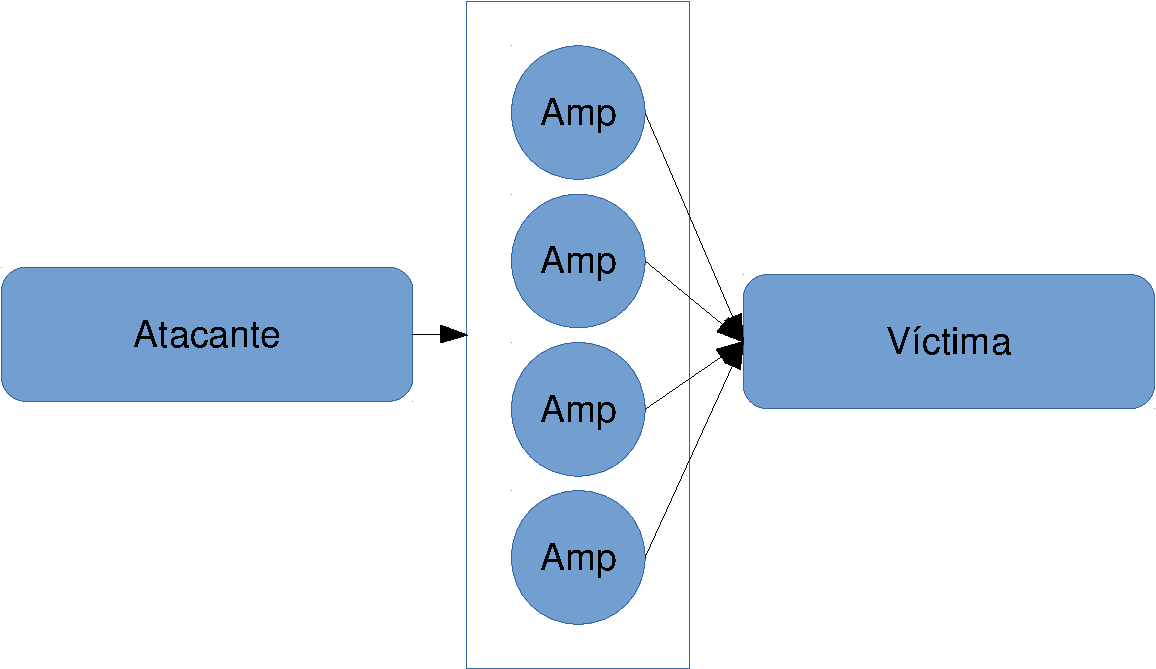
\includegraphics[width=.8\textwidth]{CapituloDDoS/Figuras/Amplificacion}
\caption{Ataque por amplificación}
\LABFIG{amplificacion} %Esto es una forma propia de los autores de gestionar las etiquetas y referencias
\end{figure}
%

Normalmente, este tipo de ataques utilizan la dirección de difusión o broadcast\index{Broadcast} \index{Difusión}. La 
dirección de difusión es una dirección especial en las redes en las que todos los nodos recibirán el paquete. Si ese 
paquete es una petición que requiere una respuesta, y tiene como dirección origen la dirección IP\index{Dirección IP} 
de la víctima (IP spoofing\index{IP Spoofing}), todos los nodos de la red responderán el mensaje, saturando la máquina 
objetivo.

Un ejemplo sencillo de este tipo de ataque es el denominado Ataque \emph{Smurf}\index{Smurf}, que utiliza un 
simple \gls{ICMP}\index{ICMP} PING\index{ICMP}\index{PING}. Si a todos los nodos de la red les llega una petición de PING 
proveniente de la dirección de la víctima, la víctima se encontrará con tantas respuestas como nodos configurados para 
responder tenga la red. Dichas respuestas tendrán que ser, al menos, procesadas por el sistema operativo de la máquina 
objetivo, que terminará saturando. Por otro lado, el contenido de la respuesta será una copia del contenido de la 
petición, por lo que es sencillo multiplicar (amplificar) el ancho de banda consumido por la víctima emitiendo un 
paquete grande.

Una variante del anterior es el ataque \emph{Fraggle}. El protocolo \gls{UDP}\index{UDP} tiene su propio sistema de PING, en 
el puerto 7. Además, tiene un sistema de generación de cadenas aleatorias en el puerto 19, el cual envía cadenas de 
texto aleatorias de longitud aleatoria (pero reducida) cualquiera que las pida. De nuevo, la mecánica del ataque es 
falsear la dirección de origen para que estos servicios respondan a la víctima, saturando así la capacidad de sus 
recursos.

\paragraph{Ataques reflejados}\mbox{\newline} \index{Ataques reflejados}

\noindent Para este apartado, un reflector es un nodo que responde a un paquete con otro paquete destinado a la 
dirección origen del primer paquete. Así, podríamos englobar en este apartado, por ejemplo, servidores \gls{DNS}\index{DNS}. 
Ver \FIG{reflexion}.

\begin{figure}[htbp]
\centering
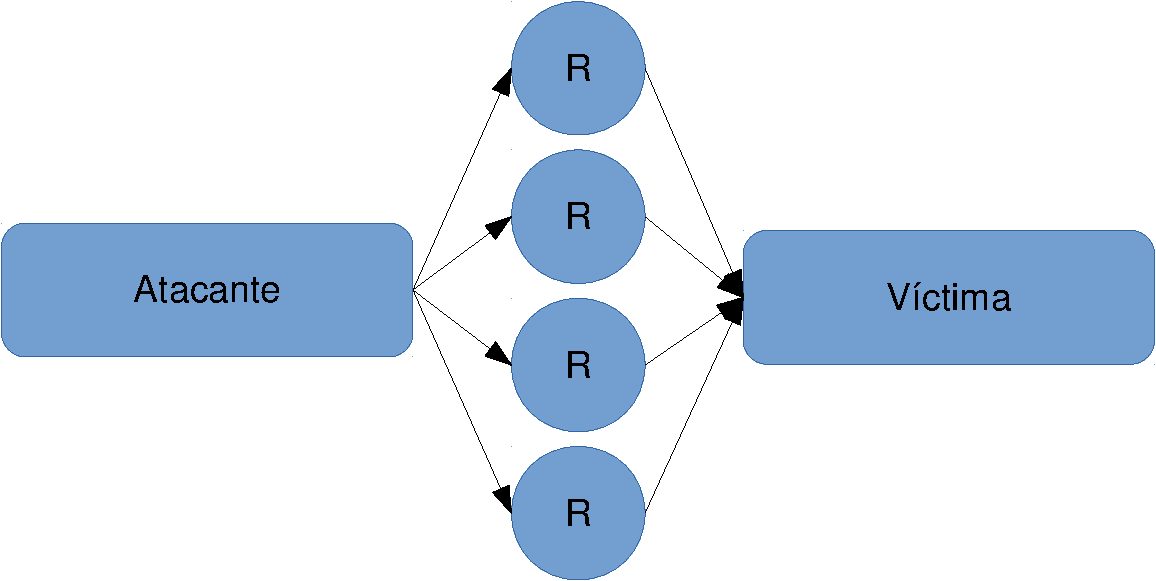
\includegraphics[width=.8\textwidth]{CapituloDDoS/Figuras/Reflexion}
\caption{Ataque por reflexión}
\LABFIG{reflexion} %Esto es una forma propia de los autores de gestionar las etiquetas y referencias
\end{figure}
%

El atacante, entonces, crea una lista de IP reflectoras, y envía para el ataque una petición a cada una de las 
direccionas, con dirección origen la de la vícima. De esta forma, localizar y detener el ataque se vuelve mucho más 
difícil, ya que, siguiendo el ejemplo, cada servidor \gls{DNS} tiene un dirección IP que no tiene nada que ver con el resto.

Sin embargo, nada impide, en principio, combinar este ataque con el tipo amplificación (por ejemplo, si se 
disponen de muchos \gls{DNS} en la misma subred). Por otra parte, es posible hacer una petición recursiva a un servidor \gls{DNS}, 
de forma que en la respuesta viaja el resultado de cada servidor \gls{DNS}. Esto es, con una pequeña petición (cabecera \gls{UDP}, 
\gls{DNS} y nombre de dominio pedido) obtenemos una respuesta mucho mayor, y ya dirigida a la dirección de la victima. 

Así pues, la diferencia entre este tipo y el anterior es que el atacante necesita de una lista de direcciones de host, 
e ir iterando para conseguir el efecto deseado, mientras que en la otra cada paquete se amplificaba mediante el uso de 
la difusión.

\paragraph{Ataques basados en botnets}\mbox{\newline}

\noindent Un bot o zombi es un equipo infectado y controlado remotamente por un maestro. Éste puede ser usado para 
enviar correo no deseado, distribuir malware, espiar (esnifar\index{Esnifar tráfico}) tráfico o, en nuestro caso de 
estudio, para perpetrar un ataque de denegación de servicio. 

Gracias a la red de zombis, el atacante real es mucho más difícil de localizar, además de servir como una primera etapa 
de amplificación del ataque.

\subsubsection{DoS Semánticos}\LABSSSEC{DDoS semanticos}
Esta segunda forma de ataque no se basa en la fuerza bruta o en la extenuación de recursos, sino en 
provocar que el servidor\footnote{O algún elemento de la infraestructura de la comunicación} entre en un estado 
\emph{ilegal}, de forma que no pueda ofrecer el servicio. No es necesario un atacante (o varios) con mucha fuerza, sino 
que se puede llevar a cabo con muy pocos recursos. Sin embargo, requiere un conocimiento mucho más profundo del 
servidor y canal de comunicación. Eso sí, el ataque es más sutil y, lo más importante, puede ser corregido con una 
adecuada configuración o actualización de componentes.
 
Uno de los principales ataques de este estilo consiste en enviar información concreta que sabemos de antemano que 
provocará una caída o malfuncionamiento en el servidor, es decir, aprovechando un fallo de seguridad. Por ejemplo, hasta 
hace relativamente poco (1997), el famoso \emph{ping de la muerte}\index{Ping de la Muerte} \cite{Bidou} era capaz de 
tumbar un servidor con tan sólo un comando: \texttt{ping <objetivo>\ -l 65511}, el cual viene integrado en todos los 
sistemas operativos. Éste aprovechaba que la pila \gls{ICMP} asumía que el paquete tenía una longitud determinada. Al 
procesar el paquete, y superarse esta longitud, se producía un desbordamiento de buffer que hacía que el servidor 
colapsase.

Otro ejemplo de ataque de este tipo es el ataque \emph{land\index{Land attack}}. En él, la victima recibe un paquete 
\gls{TCP} cuya dirección origen y destino es él mismo, por lo que intenta contactar consigo mismo hasta que colapsa. 

El ataque \emph{\index{Teardrop}} también es muy famoso, consistente en enviar mensajes IP fragmentados y malformados a 
la máquina objetivo. De esta forma, al intentar des-fragmentarlos, la máquina colapsa.

Las nuevas tecnologías tampoco son inmunes a este tipo de ataque. \gls{IPv6}, por ejemplo, puede sufrir de 
\emph{Anuncio de vecino envenenado\index{Neighbour Advertisement Spoofing Attack}}. En él, un equipo intermedio se 
anuncia como poseedor de una dirección en el camino del cliente al servidor (o bien, la dirección del propio servidor), 
y anuncia su dirección \gls{MAC} para que todos los paquetes destinados al servidor le lleguen a él. Esto es, es la 
versión \gls{IPv6} del \gls{ARP} spoofing\index{ARP Spoofing}.

\subsection{Objetivo del ataque}
Si queremos ser capaces de defendernos ante un ataque \gls{DDoS}, es necesario conocer a qué objetivos van destinados. 
De esa 
forma, podremos centrarnos en defender los activos vulnerables de una forma eficiente.

Podemos clasificar los ataques según el nivel de la capa \gls{OSI} que atacan en ataques a los routers, a la red, al 
SSOO o a la propia aplicación. Obviamente, un ataque a un nivel inferior afectará a todos los niveles superiores.

\subsubsection{Ataque a dirigido a redes}
La red es el componente más básicos de los ataques DDoS. Si el cliente es incapaz de conectar con la red del servicio, 
es imposible que éste pueda ser ofrecido. Por su parte, si la red del servicio está saturada, ningún cliente será capaz 
de acceder a la misma.

Para agravar las cosas, las aplicaciones confían cada vez más en servicios dependientes de la red. Ejemplo de ello es 
la proliferación de servicios web\index{Servicio Web} (aquellos que usan el protocolo \acrshort{HTTP} para su 
funcionamiento), o los servicios en la nube\index{Servicio en la nube} (esto es, aquellos en los que el almacenamiento 
y procesado de datos se realiza en ordenadores remotos, a los que se accede por Internet). 

No solo las redes corporativas exponen sus servicios a Internet. Poco a poco, sistemas críticos, tales como plantas 
generadoras de energía o de procesado de agua, están dentro de una red que, a su vez, en unos pocos saltos están 
conectadas a Internet. De esta forma, estos servicios podrían ser víctimas de un ataque \gls{DDoS}. Es posible, 
incluso, que el lanzar un ataque hacia otro servicio en esta red intermedia afecte a dicho servicio crítico 
\cite{Raghavan}.

Así pues, un ataque de denegación de servicio que afectase a dicha infraestructura crítica podría tener repercusiones 
muy serias, tales como dejar sin energía o agua una zona del mapa, y que pocos sistemas escapan actualmente de la 
posibilidad de un ataque \gls{DDoS}: En el momento que lo conectas a Internet, estás expuesto a ello.

Uno de los protocolos más usados para el transporte de información es \gls{TCP}, por lo que un gran porcentaje de 
ataques van dirigidos contra esta tecnología.

\paragraph{Reseteo de conexiones}\mbox{\newline}

Un ataque muy simple consiste en, una vez que el atacante conoce una conexión existente, reiniciar dicha conexión. Una 
conexión en \gls{TCP} está identificada por una dirección origen, una dirección destino, un puerto origen y un puerto 
destino. Existe un bit RST\index{TCP RST} en la cabecera \gls{TCP} que permite reiniciar una conexión inmediatamente. 
Esto es usado, por ejemplo, si uno de los dos extremos detecta un problema en la conexión. Para terminar de empeorar 
las cosas, RST no necesita \gls{ACK}, por lo que el cliente no llega a saber que la conexión ha terminado

Tras recibir el servidor el RST, el cliente continúa enviando paquetes, y se encontrará con un socket cerrado. El 
servidor enviará otro RST, y será imposible mantener la conexión durante un largo periodo de tiempo. 

Si el atacante ha conseguido localizar una conexión, y es capaz de enviar un paquete \gls{TCP} con dicho bit activo, el 
receptor de dicho paquete no aceptará más paquetes de esa conexión, y, por tanto, se habrá conseguido que la conexión 
quede invalidada. Podemos ver una descripción gráfica de este ataque en la \FIG{RST attack}.

\begin{figure}[htbp]
\centering
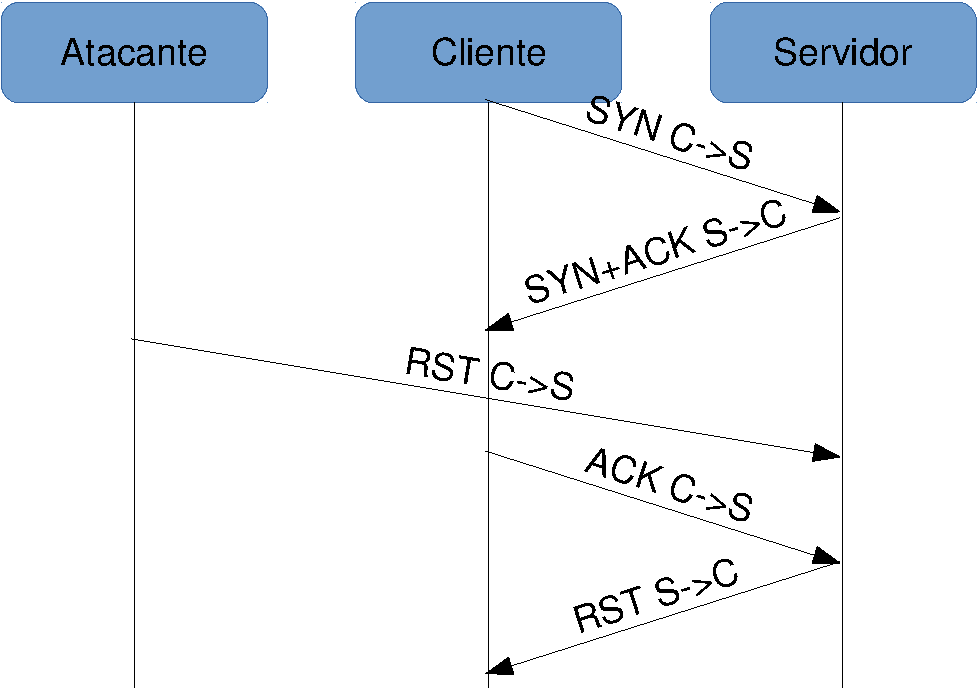
\includegraphics[width=.8\textwidth]{CapituloDDoS/Figuras/RST_attack}
\caption{Ataque RST}
\LABFIG{RST attack} 
\end{figure}
%

\paragraph{Asentimientos optimistas}\mbox{\newline}

Otra característica comúnmente explotada de las conexiones \gls{TCP} es su control de congestión\index{Control de 
congestión TCP}. Para calcular la saturación del enlace, un extremo considera como paquete perdido (y, por tanto, el 
enlace está saturado) aquel paquete que tarda más de $T$ segundos en recibir el ACK. Al iniciar la conexión \gls{TCP}, el 
algoritmo de arranque lento\index{TCP Slow Start} incrementará el número de paquetes enviados de una forma exponencial.

Si el atacante envía \gls{ACK} optimistas, esto es, \gls{ACK} de un paquete que realmente no ha recibido aún, el atacante enviará 
cada vez más y más paquetes salientes, hasta saturar su conexión. Teniendo en cuenta que un \gls{TCP} \gls{ACK} sólo ocupa 54 
bytes, el efecto amplificador de este tipo de ataque es bastante importante. Algunos estudios hablan de que, con una 
conexión de $56kbps$, es posible generar en el lado del atacante unos $8.9mbps$ \cite{sherwood}.

Podemos ver un ejemplo de este tipo de ataques en la \FIG{optim ACK attack}.

\begin{figure}[htbp]
\centering
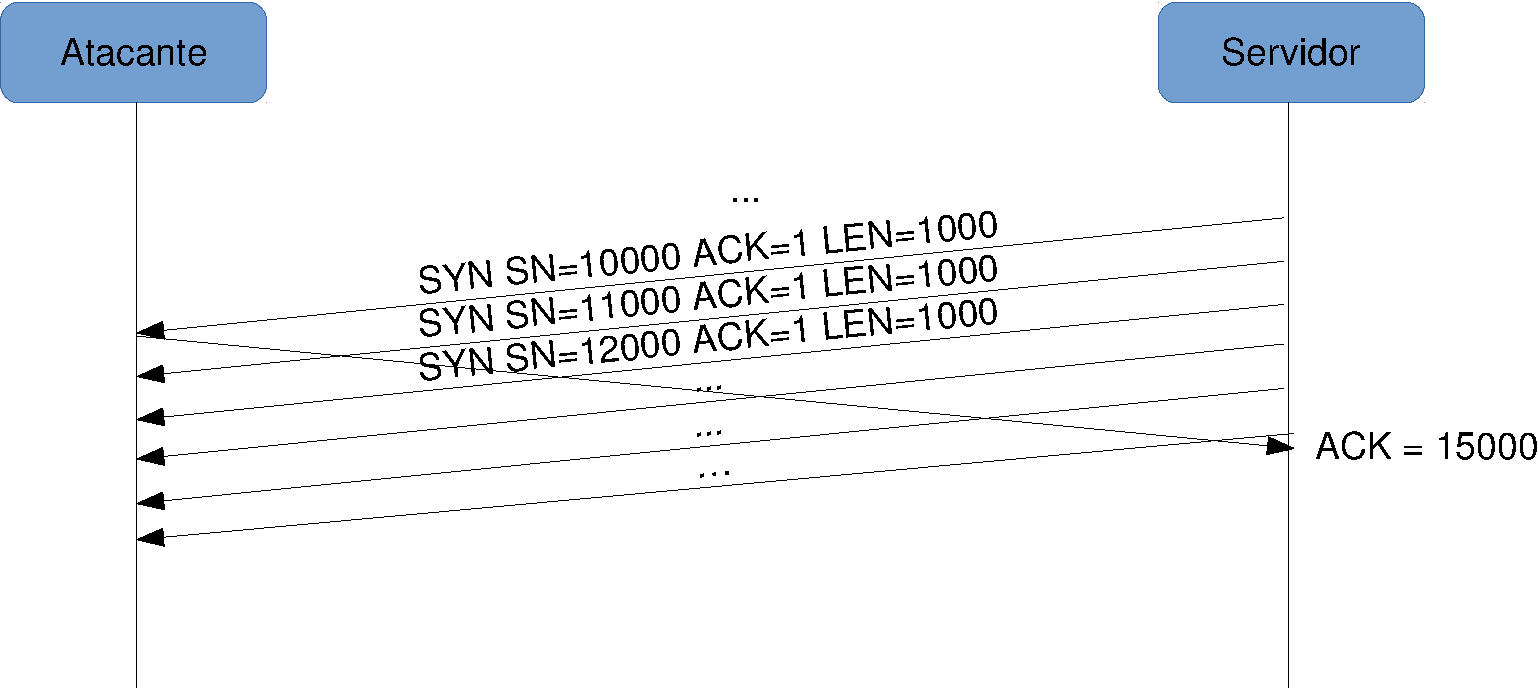
\includegraphics[width=\textwidth]{CapituloDDoS/Figuras/optim_ACK_attack}
\caption{Ataque por ACK optimista}
\LABFIG{optim ACK attack} 
\end{figure}
%

\paragraph{Temporizador de retransmisión}\mbox{\newline}

Cuando un paquete se pierde en una conexión \gls{TCP}, el protocolo dice que es necesario reenviarlo. Como ya hemos 
explicado, un paquete perdido es aquel que no recibe el \gls{ACK} correspondiente.

El atacante podría saturar los dispositivos de comunicación si envía una gran inundación de paquetes a los mismos. Sin 
embargo, esto sería fácilmente detectable por dispositivos que monitorizan la red.

En su lugar, el atacante enviará una ráfaga de corta duración pero de mucha intensidad, lo suficiente para saturar los 
dispositivos y hacer perder paquetes. En este caso, \gls{TCP} alcanzará el estado de \emph{timeout} en todas las 
comunicaciones, y necesitará comenzar a retransmitir los paquetes por donde iba la conexión.

Siguiendo el procedimiento de \gls{TCP}, se debe comenzar a retransmitir los paquetes en ráfagas, empezando por un 
paquete por ráfaga e ir aumentando progresivamente. En poco tiempo, se debería volver a alcanzar un buen ritmo para la 
conexión.

Sin embargo, si el atacante, al acabar el temporizador de retransmisión, vuelve a lanzar otro ataque intensivo pero de 
corta intensidad y vuelve a saturar los elementos de comunicación, las conexiones no serán capaces de recuperarse.

Así pues, el atacante ha aprovechado el propio tiempo de retransmisión \gls{TCP} para dejar incomunicado el servidor, y 
de esa forma amplificar su ataque: Con ráfagas cortas, es capaz de producir el mismo efecto que si saturase el canal 
continuamente. Menos ancho de banda consumido, y menos probabilidades de detección.

En la \FIG{RTO attack} podemos ver el perfil que tendría el tráfico atacante para bloquear la comunicación. En ella, 
$I_p$ es la intensidad del pico del ataque, $T_p$ es la duración del pico atacante, y $T_{timeout}$ es el temporizador 
de retransmisión que tiene \gls{TCP}.

\begin{figure}[htbp]
\centering
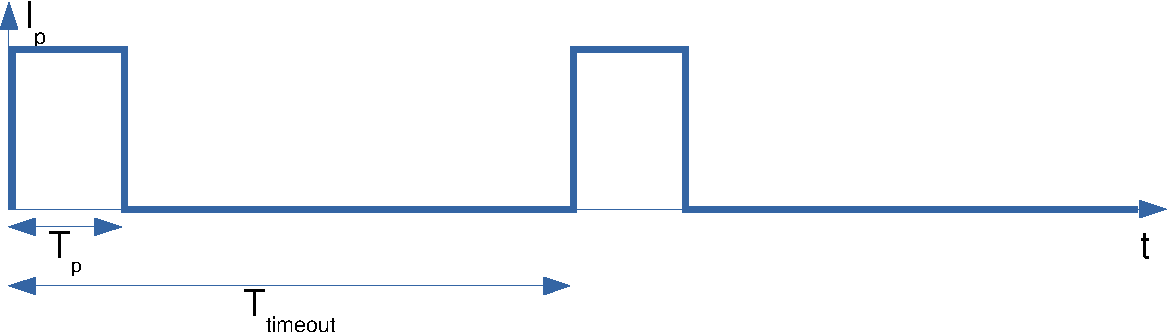
\includegraphics[width=\textwidth]{CapituloDDoS/Figuras/RTO_attack}
\caption{Ataque por retransmisión TCP}
\LABFIG{RTO attack} 
\end{figure}
%

\subsubsection{Ataque a Sistemas Operativos}\LABSSSEC{Ataques a SSOO}

El encargado de transportar correctamente los paquetes desde la red hasta la aplicación. Si el atacante es capaz de 
hacer que este intermediario no sea capaz de llevar los paquetes desde o hacia la aplicación, habrá logrado llevar a 
cabo un ataque \gls{DoS}.

En este tipo de ataque se busca explotar una vulnerabilidad en el modo que el \gls{SO} gestiona los paquetes. Por 
ejemplo, si a la hora de recibir un paquete, el \gls{SO} lo escribe en memoria sin comprobar los límites de la memoria 
reservada para ello, el atacante podría enviar un paquete lo suficientemente largo como para provocar un \emph{Buffer 
Overflow}\index{Buffer Overflow}, esto es, se escribirá en una zona de memoria indebida, provocando que el sistema 
colapse. Esta técnica es la empleada por el llamado \emph{ping de la muerte}\index{Ping de la Muerte}, ya explicado en 
el \SSSEC{DDoS semanticos}.

Otro ataque, también dirigido a saturar el \gls{SO}, sería un \emph{\gls{SYN} Flood} (inundación \gls{SYN}). Esta vez, 
con la inundación, no provocamos saturar la red, sino la capacidad de conexiones simultaneas que aguante el sistema.

\subsubsection{Ataques dirigidos a aplicaciones (Ataques capa 7)}

Muchas aplicaciones están desarrollando sus aplicaciones sobre una arquitectura tipo servicio web, esto es, programas 
distribuidos que funcionan mediante el paso de mensajes sobre el protocolo HTTP. Para que este servicio funcione, si 
está expuesto a Internet, es necesario que el cortafuegos permita el tráfico hacia esa aplicación. Por tanto, el 
atacante es capaz también de alcanzar dicho servicio, aunque quizás no pueda usarlo por necesitar, por ejemplo, unas 
credenciales válidas.

Al igual que los servicios web, la aplicación distribuida puede estar confiando en cualquier otro tipo de tecnología 
subyacente. Mientras que esta se encuentre en espacio de usuario, se considerará un ataque de capa 7.

Los métodos para realizar este ataque son muy parecidos a los de la \SSSEC{Ataques a SSOO}. Por la parte semántica, se 
puede intentar enviar información corrupta que haga al servidor entrar en un estado incorrecto, que no pueda continuar 
sirviendo. Por otra parte, tenemos los ataques por inundación, que buscarían saturar la capacidad del servidor, y que 
a la máquina le sea imposible seguir respondiendo peticiones.


\section{Técnicas de detección y mitigación de un ataque DDoS}\LABSEC{Deteccion y mitigacion DoS}
\subsection{Ataques por inundación}
La principal señal que indica que un servicio está sufriendo un ataque por inundación es que reciben una cantidad de 
tráfico anormalmente grande. Sin embargo, para una detección correcta deberíamos definir qué supone \emph{anormal}. 

La necesidad de esa definición de lo que supone un tráfico normal y lo que no se ve claramente con el ataque tipo 
\emph{Efecto slashdot}. Lo que para el tráfico del servidor de noticias es algo normal, es un volumen completamente 
inadmisible para un servidor pequeño, y logrará tumbarlo rápidamente.

A lo largo de este trabajo intentaremos definir un sistema de detección de anomalías (CUSUM, \CHAP{Algoritmo CUSUM}), y 
qué parámetros debemos usar para buscar un compromiso entre velocidad de detección y no aparición de falsos positivos.

Para mitigar el ataque, no basta con cortar el acceso al servicio, ya que entonces el \gls{DDoS} habría triunfado. Es 
necesario discernir entre las direcciones IP maliciosas o atacantes, y cortar el tráfico sólo a ellas, permitiendo que 
las direcciones benignas sigan navegando como hasta ahora.

\subsection{Ataques semánticos}
Para la detección de ataque ssemánticos, el método más usado es la detección de patrones. Esto es, analizar el paquete 
en busca de características del mismo que detecten que estamos ante un paquete, al menos sospechoso. Al patrón que 
siguen esos paquetes maliciosos y que, por tanto lo hace detectable, se le denomina \emph{firma}\index{Firma}.

Por ejemplo, en el caso del \emph{ping de la muerte}, un sistema intermedio podría analizar todos los paquetes que van 
hacia el servidor y, en caso de ser de un tamaño superior o igual a $2^16=65536$, bloquar el paso de dicho paquete.

Comparativamente hablando, tienen la desventaja de necesitar la constante actualización de la base de datos de firmas, 
y la posibilidad de que esta base de datos crezca, haciendose más inmanejable. Su refinamiento consiste en la selección 
de reglas adecuadas a los activos protegidos, esto es: Si no tengo un servidor web, no necesito estar analizando 
paquetes contra firmas que comprometen servidores web, es un gaso inútil.

Este es el sistema de detección usado por IPS tales como snort \cite{snort} o suricata \cite{suricata}. A lo largo de 
este trabajo no pretenderemos abarcar este tipo de soluciones.

\section{Conclusiones}
Así pues, un ataque de \gls{DoS} es cualquier cosa que permita que un servicio deje de estar disponible. 
Como consecuencia, los posibles beneficios que ese servicio pudiese estar generando se ven anulados, y es posible que 
algunos usuarios dejen de confiar en él.

Podríamos dividirlos entre ataques por inundación, en los que englobaríamos aquellos que persiguen agotar los recursos 
en los que se apoya el servicio, o bien ataques semánticos, que buscan explotar alguna vulnerabilidad encontrada en los 
mismos. La forma efectiva de detectar dichos ataques es, respectivamente, el análisis de flujos de tráfico, y el 
análisis de paquetes en busca de firmas o patrones conocidos.

Los ataques de denegación de servicio pueden ir destinados a agotar o explotar vulnerabilidades de cualquier capa en la 
que se apoye el servicio. Esto es, pueden atacar al propio servicio, o bien al \gls{SO} sobre el que es ofrecido, o a 
cualquier elemento de red entre el usuario y el servicio. Si logra inutilizar un elemento de capa baja, todos los 
elementos superiores caen en efecto cascada.

Por último, es posible realizar el ataque desde muchos puntos distintos, esto es, haciendo que el ataque sea 
perpetrado por muchos atacantes distintos. De esta forma, conseguimos aumentar la magnitud del ataque y dificultamos 
la supervivencia del servicio. Cuando esto ocurre, estamos hablando de un ataque \gls{DDoS}.


\section{Resumen}%%%%%%%%%%%%%%%%%%%%%%%%%%%%%%%%%%%%%%%

\begin{Resumen}[Resumen del capítulo]
\subsection*{Definición}
Acción(es) que impiden que un sistema de información funcione normalmente. 

\subsection*{Taxonomía}
\begin{flalign*}
 &\begin{cases}
   \text{Por inundación.}
   \begin{cases}
     \text{Coordinados por seres humanos / manuales.}\\
     \qquad\text{\emph{Ningún elemento automático}}\\
     \text{Amplificados.}\\
     \qquad{\text{\emph{El atacante sólo envía N y el ataque se amplifica}}}\\
     \qquad{\text{\emph{Ejemplo: ping a direcciones broadcast}}}\\
     \text{Reflejados.}\\
     \qquad{\text{\emph{El atacante tiene una lista de IP que pueden reflejar su ataque}}}\\
     \qquad{\text{\emph{Ejemplo: Peticiones DNS con dirección origen de la víctima}}}\\
     \text{Botnets o redes Zombi.}\\
     \qquad{\text{\emph{Efecto amplificador y ocultador}}}
     \text{Combinación de las anteriores.}
   \end{cases}\\
   \text{Semántico.}\\
   \qquad{\text{\emph{Se busca explotar fallos}}}
 \end{cases}&
\end{flalign*}

\subsection*{Objetivo del ataque}
\begin{flalign*}
 &\begin{cases}
   \text{Dirigido a redes.}\\
   \qquad{\text{\emph{Ejemplos:}}}
   \begin{cases}
     \text{Reseteo de conexiones.} \\
     \text{Asentimientos optimistas.} \\
     \text{temporizador de retransmisión.} \\
   \end{cases}\\
   \text{Ataques a SSOO.} \\
   \text{Ataques de capa 7.}\\
 \end{cases}&
\end{flalign*}

\subsection*{Técnicas de detección y mitigación}
\begin{flalign*}
 &\begin{cases}
   \text{Por inundación.}
   \begin{cases}
     \text{Detección de comportamiento \emph{anómalo} en la red.} \\
     \qquad\rightarrow\text{¿Definición de anómalo?} \\
     \text{Bloqueo de direcciones con comportamientos anómalos}\\
     \qquad\rightarrow\text{Posibilidad de falsos negativos y falsos positivos}\\
     \text{Tuneado consistente en definir \emph{normal}}
   \end{cases}\\
   \text{Semánticos}
   \begin{cases}
     \text{Detección de patrones (firmas) en el tráfico.} \\
     \qquad\rightarrow\text{Necesidad de actualización} \\
     \text{Bloqueo de paquetes que cumplan dichos patrones}\\
     \qquad\rightarrow\text{Posibilidad de falsos negativos y falsos positivos} \\
     \text{Tuneado consiste en seleccionar reglas en base a los activos a proteger}
   \end{cases}
 \end{cases}&
\end{flalign*}

\end{Resumen}

